%!TEX root = ../Thesis.tex
\section{Guidance Simulations} % (fold)
\label{sec:guidance_simulations}
This section presents the results from the simulations of the Parallel Navigation- and Model Optimal Guidance methods discussed in section \ref{sec:guidance_methods}. The weighting matrices $\vect{Q}$ and $\vect{R}$ used in the simulations presented are given in \ref{eq:sim_mat_QR}, the constraints restricting the states are given in \ref{eq:sim_const_x} and the constraints limiting the input are given in \ref{eq:sim_const_u}.
\begin{align}\label{eq:sim_mat_QR}
	\vect{Q}&=
	\begin{bmatrix}
		1.3&0&0&0\\
		0&1.3&0&0\\
		0&0&500&0\\
		0&0&0&500
	\end{bmatrix}
	&
	\vect{R}&=
	\begin{bmatrix}
		0&0&0&0\\
		0&0&0&0\\
		0&0&1&0\\
		0&0&0&1
	\end{bmatrix}
\end{align}
\begin{align}\label{eq:sim_const_x}
	\vect{x}^{low}
	&=
	\begin{bmatrix}
		-\infty\\
		-\infty\\
		-\infty\\
		-\infty
	\end{bmatrix}
	&
	\vect{x}^{high}
	&=
	\begin{bmatrix}
		\infty\\
		\infty\\
		\infty\\
		\infty
	\end{bmatrix}
\end{align}
\begin{align}\label{eq:sim_const_u}
		\vect{u}^{low}
	&=
	\begin{bmatrix}
		u^n_{d/u,x,k}\\
		u^n_{d/u,y,k}\\
		-15\\
		-15
	\end{bmatrix}
	&
	\vect{u}^{high}
	&=
	\begin{bmatrix}
		u^n_{d/u,x,k}\\
		u^n_{d/u,y,k}\\
		15\\
		15
	\end{bmatrix}
	&
	\vect{\Delta u}
	&=
	\begin{bmatrix}
		\infty\\
		\infty\\
		2.5\\
		2.5
	\end{bmatrix}
\end{align}
where the states inequality constraints \ref{eq:sim_const_x} gives no restrictions in the flight area. The control constraints in \ref{eq:sim_const_u} restricts the \gls{UAV} velocity to $\pm15m/s$ and forces the optimization algorithm to predict constant velocity equal to the measured velocity $u^n_{d/u,k}$ on the control objective. 

Figure~\ref{fig:variousPredLen} illustrates how the behavior of the Optimal Guidance Controller changes by using different prediction lengths $N$.
\begin{figure}[ht!]
\centering
	\begin{subfigure}[b]{.5\textwidth}
		\centering
		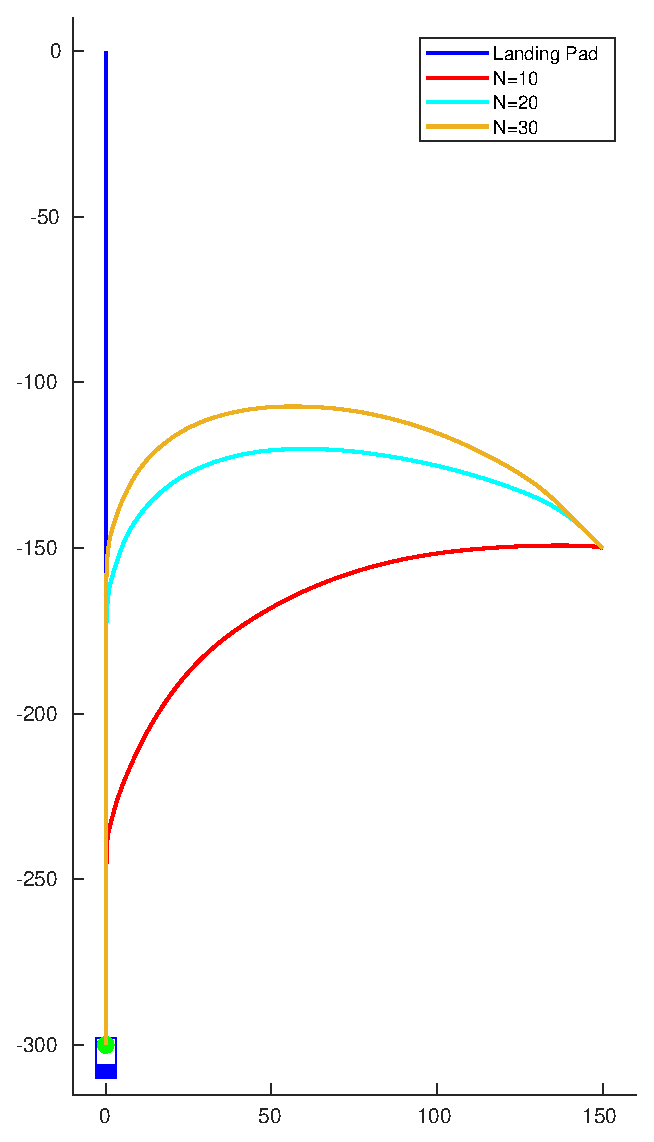
\includegraphics[width=\linewidth]{img/plot/simulation/pred_length.eps}
		\captionof{figure}{Position track from the LP and UAV's}
		\label{fig:variousPredLen_pos}
	\end{subfigure}%
	\begin{subfigure}[b]{.5\textwidth}
		\centering
		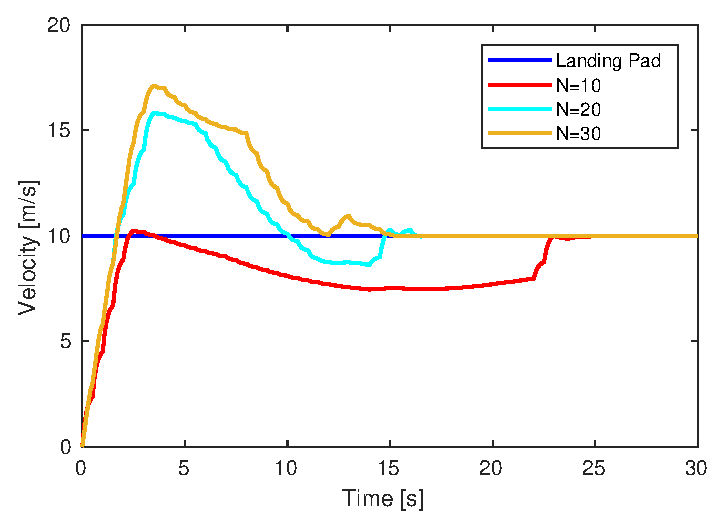
\includegraphics[width=\linewidth]{img/plot/simulation/pred_length_vel.eps}
		\captionof{figure}{Velocity from LP and UAV's}
		\label{fig:variousPredLen_vel}
	\end{subfigure}
	\caption{Optimal Guidance with different prediction lengths}{Optimal Guidance with different prediction lengths. Constant velocity LP}\label{fig:variousPredLen}
\end{figure}
Where the blue line in sub figure~\ref{fig:variousPredLen_pos} represents the path driven by the landing pad at constant velocity and the remaining lines represents the path driven by the UAV using Optimal Guidance controller with different prediction lengths. Sub figure~\ref{fig:variousPredLen_vel} presents the velocity during the simulation. Further on in the guidance simulations, the prediction length is set to $N=10$. The parameters used in the Parallel Navigation Guidance controller are given in \ref{eq:PNG_parameters}.
\begin{align}\label{eq:PNG_parameters}
	\Delta&=16
	&
	U_{c,max}&=10
\end{align}

\subsection{Constant Velocity} % (fold)
\label{sub:constant_velocity}
The simulation results given in figure~\ref{fig:constant_vel_target} presents the behavior of the Optimal- and the Parallel Navigation Guidance tracking a target at constant velocity. There are two simulation cases presented in the figure, one where the UAV's initial positions are set to $[150,-150]$, and one where the initial positions are set to $[150,-50]$.
\begin{figure}[h!]
\centering
	\begin{subfigure}{.5\textwidth}
		\centering
		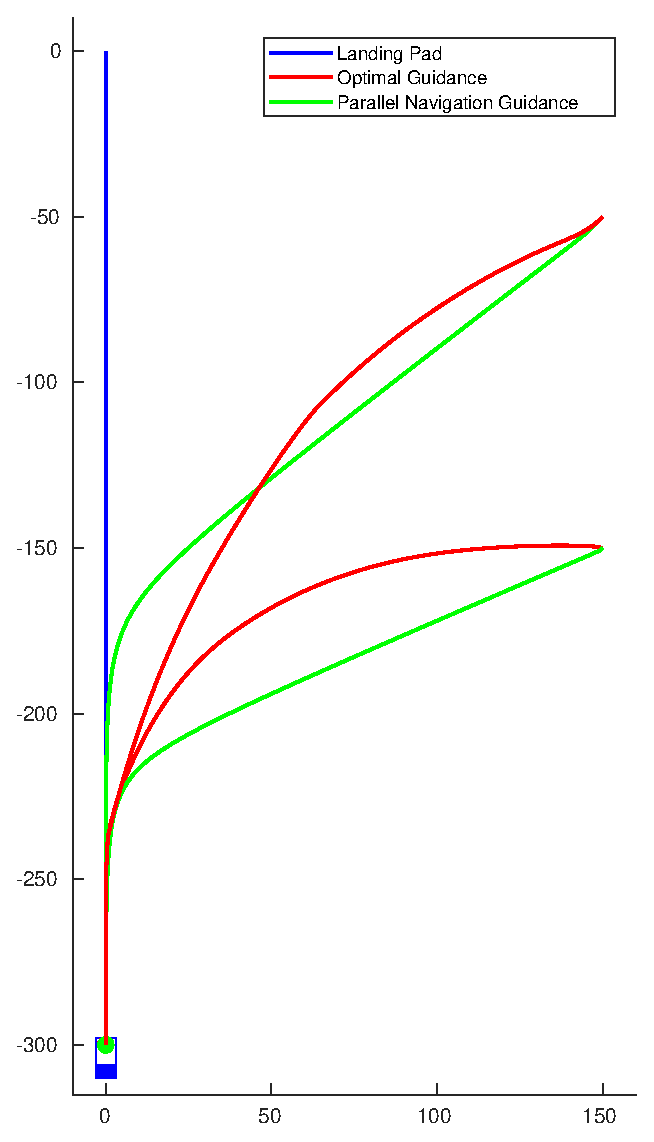
\includegraphics[width=\linewidth]{img/plot/simulation/constant_vel_two_init.eps}
		\captionof{figure}{Position track from the LP and UAV's}
		\label{fig:constVel}
	\end{subfigure}%
	\begin{subfigure}{.5\textwidth}
		\centering
		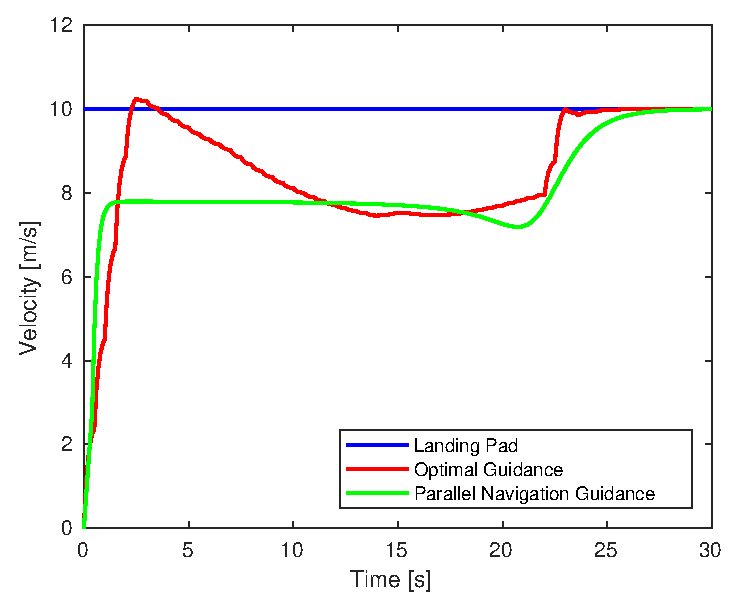
\includegraphics[width=\linewidth]{img/plot/simulation/constant_vel_two_init_vel_150.eps}
		\captionof{figure}{Initial position [150,-150]}
		\label{fig:constVel_vel_150}
		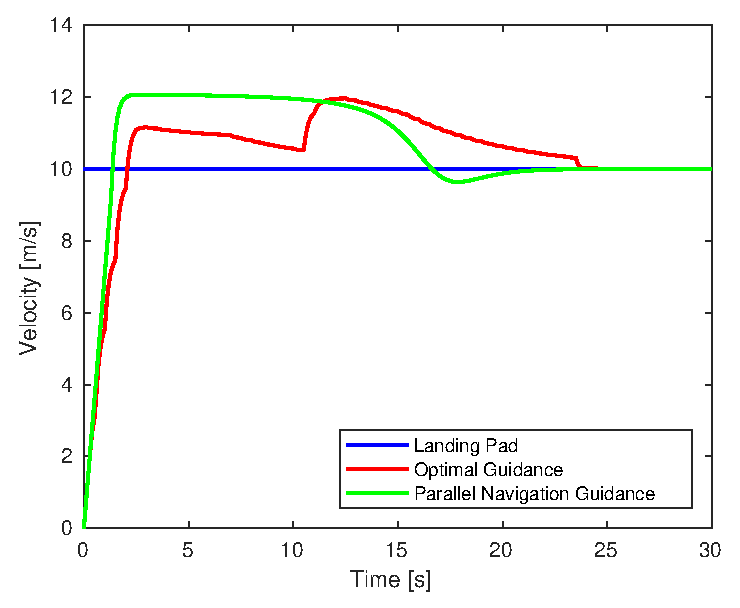
\includegraphics[width=\linewidth]{img/plot/simulation/constant_vel_two_init_vel_50.eps}
		\captionof{figure}{Initial position [150,-50]}
		\label{fig:constVel_vel_50}
	\end{subfigure}
	\caption{Optimal and Parallel navigation Guidance with a constant velocity target}\label{fig:constant_vel_target}
\end{figure}
Sub figure~\ref{fig:constVel}, illustrates the paths the UAV's and the landing pad have driven, sub figure~\ref{fig:constVel_vel_150} and \ref{fig:constVel_vel_50} illustrates the corresponding velocities using the initial condition $[150,-150]$ and $[150,-50]$ respectively.
%subsection constant_velocity (end)

\subsection{Accelerating} % (fold)
\label{sub:accelerating}
In this simulation, the landing pad is acceleration from 0 to $10m/s$ with an acceleration of $1m/s^2$ and then continues with a constant velocity. 
\begin{figure}[ht!]
\centering
	\begin{subfigure}[b]{.5\textwidth}
		\centering
		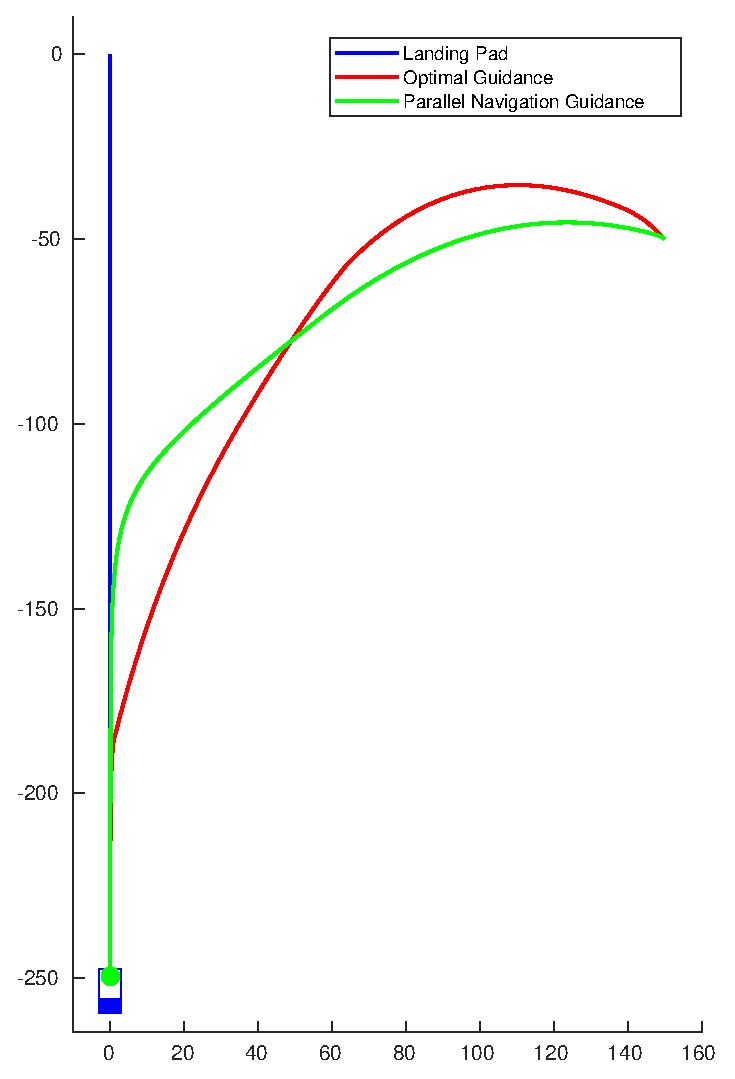
\includegraphics[width=\linewidth]{img/plot/simulation/acceleration.eps}
		\captionof{figure}{Position track from the LP and UAV's}
		\label{fig:acceleration}
	\end{subfigure}%
	\begin{subfigure}[b]{.5\textwidth}
		\centering
		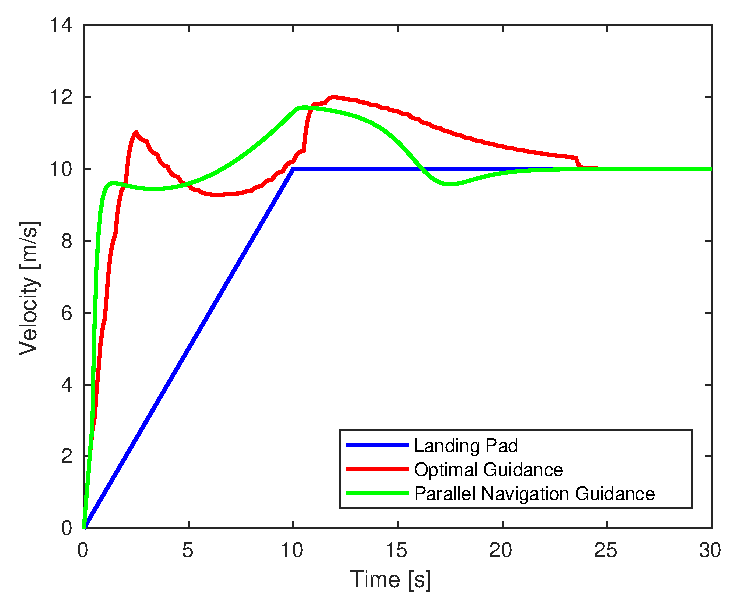
\includegraphics[width=\linewidth]{img/plot/simulation/acceleration_vel.eps}
		\captionof{figure}{Velocity from LP and UAV's}
		\label{fig:acceleration_vel}
	\end{subfigure}
	\caption{Optimal and Parallel navigation Guidance with a accelerating target}\label{fig:accel_target}
\end{figure}
Figure~\ref{fig:accel_target} presents the paths and velocities generated while tacking the landing pad using Optimal- and Parallel Navigation Guidance.
% subsection accelerating (end)

\subsection{Random Driving} % (fold)
\label{sub:random_driving}
In the simulations presented in figure~\ref{fig:rand_target}, random noise is added to the steering angle of the landing pad, while the speed is kept constant.
\begin{figure}[ht!]
\centering
	\begin{subfigure}[b]{.5\textwidth}
		\centering
		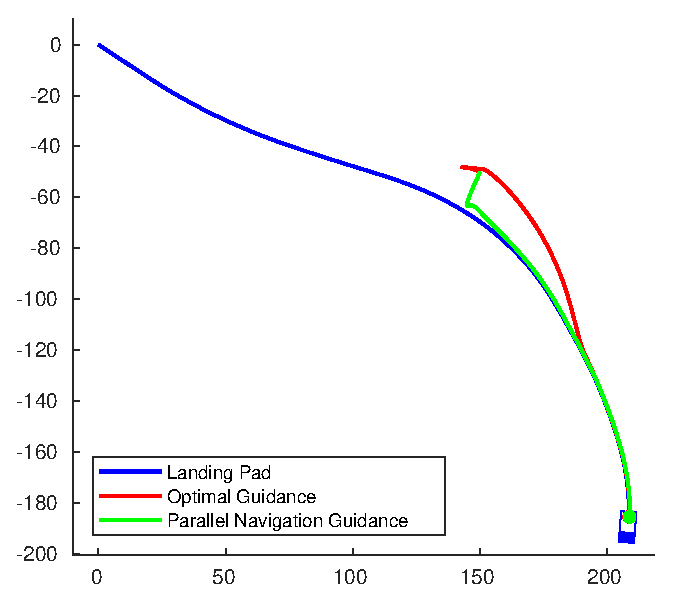
\includegraphics[width=\linewidth]{img/plot/simulation/random_1.eps}
		\captionof{figure}{Position track from random steering 1}
		\label{fig:random_1}
	\end{subfigure}%
	\begin{subfigure}[b]{.5\textwidth}
		\centering
		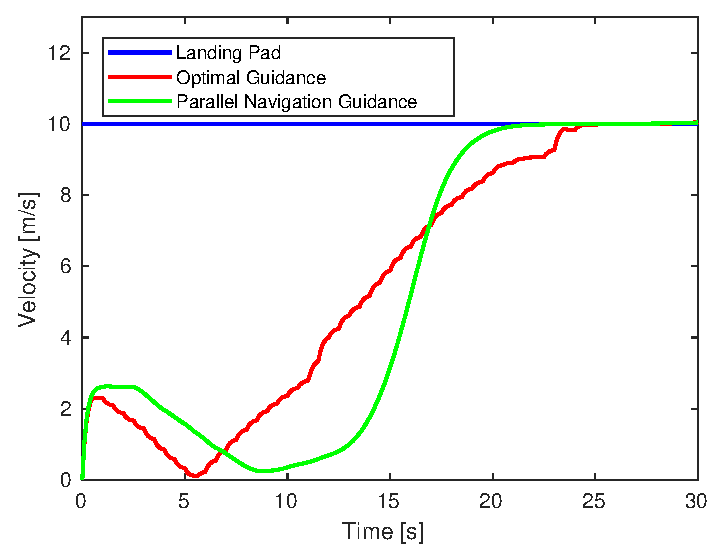
\includegraphics[width=\linewidth]{img/plot/simulation/random_1_vel.eps}
		\captionof{figure}{Velocity from random steering 1}
		\label{fig:random_1_vel}
	\end{subfigure}
	\begin{subfigure}[b]{.5\textwidth}
		\centering
		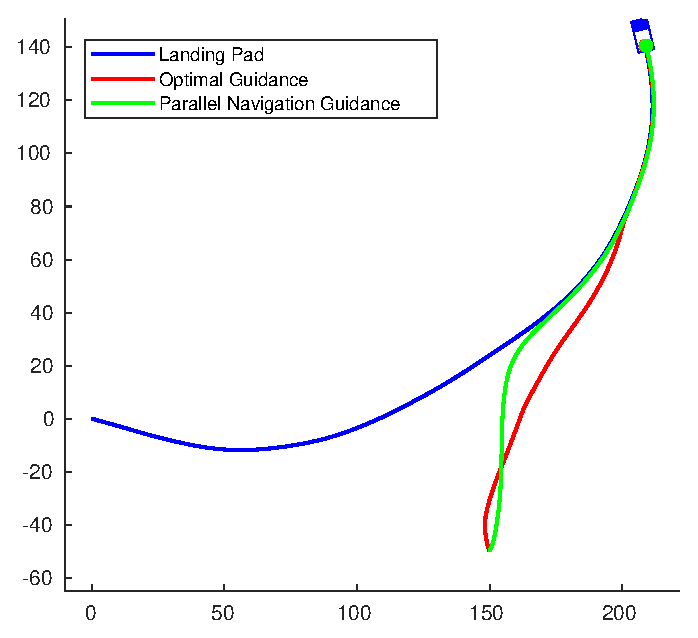
\includegraphics[width=\linewidth]{img/plot/simulation/random_2.eps}
		\captionof{figure}{Position track from random steering 2}
		\label{fig:random_2}
	\end{subfigure}%
	\begin{subfigure}[b]{.5\textwidth}
		\centering
		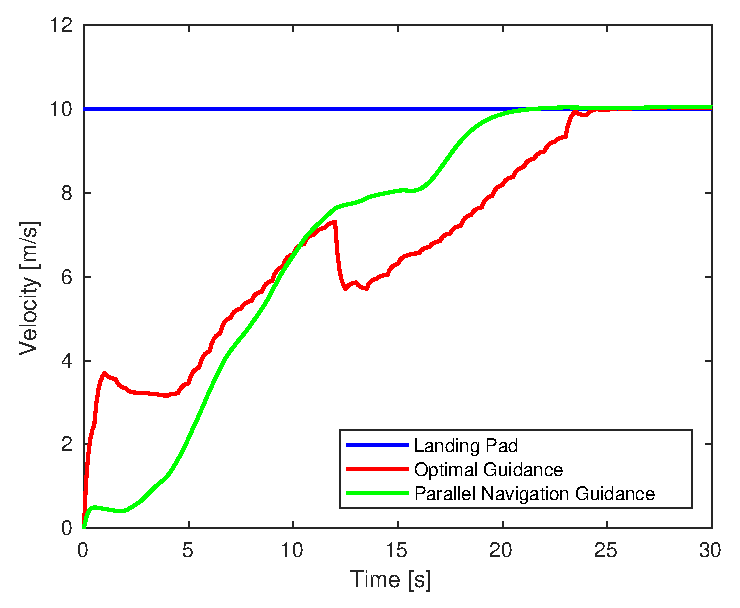
\includegraphics[width=\linewidth]{img/plot/simulation/random_2_vel.eps}
		\captionof{figure}{Velocity from random steering 2}
		\label{fig:random_2_vel}
	\end{subfigure}
	\caption{Optimal and Parallel navigation Guidance with random steering target}\label{fig:rand_target}
\end{figure}
Sub figure~\ref{fig:random_1_vel} represents the velocity of the random driving illustrated in \ref{fig:random_1}. Similarly, sub figure~\ref{fig:random_2_vel} represents the velocity from the random driving in \ref{fig:random_2}. 
% subsection random_driving (end)

\subsection{Summary} % (fold)
\label{sub:guidance_summary}
% subsection summary (end)
Overall, both the guidance methods compared in this result are able to track the desired tracking point in all the scenarios simulated. The rugged velocity measurements from the Optimal Guidance methods may be possible to smooth out by tuning the controller. However, that is one of the major disadvantage using the Optimal Guidance method. The tuning process is time consuming due to the high number of parameters to be tuned. Moreover, it is far more complex to implement and has a higher computational load compared to the Parallel Navigation Guidance method. The benefit of using the Optimal Guidance method, is the opportunity to set constraints to the states and control outputs. Such constraints can be restrictions in areas to fly, velocity and acceleration. Due to the simplicity of the Parallel Navigation Guidance method in addition to the proven stability given in section~\ref{sub:parallel_navigation_guidance}, this is the method implemented in the physical system.

% section guidance_simulations (end)